
%summary of this section.
In this section, we report on the development and verification of a complex model translation that is used to compile high level embedded system models to C programs.
We start with some background on the mbeddr language, used to prescribe software for embedded systems. Afterwards we highlight the importance that this case study has for the embedded systems that perform critical functions and how our own tool SyVolt can contribute to the development of these.
Then we give an overview of the translation that performs the compilation of mbeddr models and we show one contract that a correct compilation must satisfy. Finally, we end the section with some discussion about the limits of the SyVolt contract language.

\subsection{Mbeddr: A programming Language for Embedded Systems}

% What is mbeddr and what it is used for.
Mbeddr is a set of domain-specific extensions to the C programming language \cite{Voelter:2012:MEC:2384716.2384767}. These linguistic extensions provide well known abstractions for programming embedded systems, namely, decision tables, components and interfaces, state machines, physical units, etc\ldots
Mbeddr has been used both academically and commercially \cite{Voelter2013,Voelter2014,mry_et_al:DR:2014:4543}.

% Components
Components are a useful abstraction because they allow the embedded system modeller to separate implementation from specification.
Mbeddr allows the modeller to declare interfaces, each with a set of operation signatures (\emph{specification}). Components then can declare provided or required ports. Each port is associated with an interface thus, if a component provides a port, it must implement the operations declared in the interface of that port (\emph{implementation}). 
Instances of components communicate between each other by invocating operations through their required ports. 
These instances of components are wired together by specifying, for each required port, what provided port - and by extension the component instance that provides that port - satisfies that requirement.
The implementation of operations can be done with pure C code, decision tables and state machines.

% Decision tables
Decision tables essentially abstract nested if statements. They are a useful abstraction because one can quickly express decision making based on a large number of variables. 

% State machines
State machines abstract switch/case statements. mbeddr also provides special syntactic constructs that allow the state machine to interact with its surrounding code, for instance, react to a invocation coming through a provided port. In mbeddr, state machines can only access local variables.

% Simple example and disclaimer that the simple example is not the case study.
To make the discussion of mbeddr concrete, we introduce a simple example but please notice that this example is not the case study. The case study is the compilation of any mbeddr model to C and not just this simple example.
Listing~\ref{code:simple_example_mbeddr} shows the textual syntax\footnote{Textual syntax is an abuse. mbeddr is developed in JetBrains Meta Programming System (MPS) and MPS uses a projectional editor where the user interacts directly with the abstract syntax tree of the model with no parsing involved.} of the mbeddr model.\cgg{I have to introduce keywords to this listing to make it prettier.}


\lstset{language=C, caption={Client/Server Example in mbeddr},label=code:simple_example_mbeddr} 
\begin{lstlisting}[float]
exported cs interface Client { 
  void client_process() 
} 

exported cs interface Server { 
  string server_process(string request) 
} 

exported component Client extends nothing { 
  provides Client clientInterface 
  requires Server clientcomp_serverInterface 
   
  void clientInterface_client_process() <= op clientInterface.client_process { 
    clientcomp_serverInterface.server_process("Hello"); 
  } runnable clientInterface_client_process 
} component ClientComponent 

exported component GoodServer extends nothing { 
  provides Server serverInterface 
  string serverInterface_server_process(string request) <= op serverInterface.server_process { 
    return request; 
  } runnable serverInterface_server_process 
} component GoodServer 

exported component BadServer extends nothing { 
  provides Server serverInterface 
  string serverInterface_server_process(string request) <= op serverInterface.server_process { 
    int32 x = 0; 
    while (x >= 0) { 
      x = x + 1; 
    } while 
    return request; 
  } runnable serverInterface_server_process 
} component BadServer 

instances instances { 
  instance ClientComponent clientComponent 
  instance GoodServer gserverComponent 
  instance BadServer bserverComponent 
  connect clientComponent.clientcomp_serverInterface to gserverComponent.serverInterface
}
\end{lstlisting}

This example consists of two interfaces, three components and one instance of each component:
\begin{compactdesc}
\item[Client and Server interfaces] define the operation signatures akin to how function prototypes are defined in C.
\item[Client component] provides the Client interface through a port called ``clientInterface'' and requires the Server interface through a port called ``clientcomp\_serverInterface''. The implementation of the operation ``client\_process'', declared in the Client interface is just the invocation of the ``server\_process'' operation of the Server interface through the ``clientcomp\_serverInterface'' port.
\item[GoodServer component] provides the Server interface and the implementation of the ``server\_process'' operation is just an echo.
\item[BadServer component] provides the Server interface and the implementation of the ``server\_process'' operation is an infinite loop. The reason for this odd choice off example will become clear in the next section.
\item[Instances] are declared for each component and the required ``clientcomp\_serverInterface'' port of the Client component instance is connected to the provided ``serverInterface'' port of the GoodServer component instance.
\end{compactdesc}


\subsection{Correct Embedded Systems}

% Embedded systems need to be reliable.
The main reason for us to choose this case study is that embedded systems need to be reliable: there are industry standards such as ISO-26262, DO-178B or IEC-61508 to help ensure reliability and there are critical embedded systems such as pacemakers \cite{mry_et_al:DR:2014:4543} that also need to be correct.

% Traditional development of reliable embedded systems
Traditionally, embedded systems are implemented in C code and reliability is ensured by a combination of testing and model checking. Testing only guarantees reliability in as far as the test cases go and because C is very expressive, C programs need to be abstracted in order to properly apply model checking techniques \cite{Ivancic2005}. 
The abstraction process is error prone and time consuming as is described in \cite{Corbett2000} and \cite{Ratiu:2012:LEE:2663689.2663692}.

% Mbeddr contribution to the reliable embedded systems development
Mbeddr represents an evolution of traditional embedded system development because it starts with abstractions that can be proven to be correct and then generates C code. Model checking techniques can be applied to Mbeddr models because they contain higher level information (e.g., a state machines or decision tables) whereas with plain C code, these abstractions need to be inferred from the C.

% how does mbeddr help ensure correct embedded systems
Mbeddr is integrated with the NuSMV~\cite{Cimatti2002} model checker to perform model checking of the state machines and with the Yices~\cite{Dutertre:cav2014} Satisfiability Modulo Theories (SMT) solver to check the consistency and completeness of the decision tables.

% properties vs contracts
It is important to distinguish two types of properties: properties that a given mbeddr model needs to satisfy; and properties that all mbeddr models need to satisfy.
For instance, a property of the former type for the mbeddr model of the pacemaker system is that it never stops. A property of the later type is that decision tables, if they are used, must be consistent and complete \cite{Ratiu:2012:LEE:2663689.2663692}.

%the problems with mbeddr level of abstraction
As described in \cite{Ratiu:2012:LEE:2663689.2663692}, properties checked at the mbeddr level can only be sound if the C code that is generated satisfies the same properties as the mbeddr models.
The correctness of the C code generation is thus important to achieve soundness.
In practice this correctness is ensured by manual reviews of the code generation and automated testing.

%how can syvolt help to ensure reliability
SyVolt is a step towards ensuring the C code generation is correct automatically, provided the appropriate correctness properties (of the C code generation) are described. We will call contracts to these properties of the C code generation process.
SyVolt allows the user to express contracts that relate the generated C constructions with the elements in the mbeddr model.
This is something that cannot be done by checking the generated C code alone as it requires the traceability information between the generated C code and the mbeddr model.

%example
For instance, in SyVolt it is possible to prove that the wiring of instances of components is always respected, i.e., when executing the C code, no instance will invoke a different operation than the one that is specified in the wiring scheme at the mbeddr level. This is an important contract as it ensures, for instance, that the Client component instance in our Client/Server example (see Listing~\ref{code:simple_example_mbeddr}) will never invoke the operation of the BadServer component instance.
To see how non trivial this contract can be, look at the wiring function \verb=client_wire= of the generated code from the Client/Server example shown in Listing~\ref{code:components_sample_c}.: the wiring in the C code is done by assignment the address of the required port operation to a function pointer that is part of the instance's runtime data.
For more complex examples, this becomes very difficult to inspect in the generated code.

\lstset{language=C, caption={Client/Server Example in mbeddr},label=code:components_sample_c} 
\begin{lstlisting}[float]
struct Client_i_t {
  void (*client_process)(void*);
};
struct Server_i_t {
  char* (*server_process)(char*,void*);
};

struct Client_c_t {
  void *client_serverI_port;
  Server_i_t *client_serverI_ops;
};
struct BadServer__cdata { uint8_t aMember; };
struct GoodServer__cdata { uint8_t aMember; };

static Server_i_t bserver_serverI_ops;
static Client_i_t client_clientI_ops;
static Server_i_t gserver_serverI_ops;

static BadServer_c_t bserver_inst;
static Client_c_t client_inst;
static GoodServer_c_t gserver_inst;

char* BadServer_serverI_server_process(char *request, void *_id) 
{
  BadServer_c_t *cid = ((BadServer_c_t *)(_id));
  int32_t x = 0;
  while (x >= 0){
    x = x + 1;
  }
  return request;
}

void Client_clientI_client_process(void *_id) 
{
  Client_c_t *cid = ((Client_c_t *)(_id));
  (*cid->client_serverI_ops->server_process)("Hello",cid->client_serverI_port);
}

char* GoodServer_serverI_server_process(char *request, void *_id) 
{
  GoodServer_c_t *cid = ((GoodServer_c_t *)(_id));
  return request;
}

static void init(void) 
{
  client_wire();
  gserver_wire();
  bserver_wire();
}

static inline void bserver_wire(void) 
{
  bserver_serverI_ops.server_process = &BadServer_serverI_server_process;
}
static inline void client_wire(void) 
{_
  client_clientI_ops.client_process = &Client_clientI_client_process;
  client_inst.client_serverI_port = &gserver_inst;
  client_inst.client_serverI_ops = &gserver_serverI_ops;
}
static inline void gserver_wire(void) 
{
  gserver_serverI_ops.server_process = &GoodServer_serverI_server_process;
}
\end{lstlisting}


\subsection{Mbeddr to C Code Generation}

%small intro to this section
Listing~\ref{code:components_sample_c} already disclosed the generated C code for the Client/Server mbeddr model shown in Listing~\ref{code:simple_example_mbeddr}. However, we have not disclosed how, in general, is the C code generated from an mbeddr model.
The C code is generated with a model transformation specified between two metamodels: the source metamodel is the mbeddr metamodel and the target metamodel is the C metamodel.

\subsubsection{Source and Target Metamodels}

We present a simplified version of the mbeddr metamodel in Figure~\ref{fig:Moduleclassdiagram}:
\begin{compactdesc}
	\item[ImplementationModule] represents the root container of the mbeddr model. It is composed of InstanceConfigurations, AtomicComponents and ClientServerInterfaces. There are other kinds of interfaces but they are not relevant for our purposes.
	\item[ClientServerInterface] represents a set of Operations. An Operation represents a signature, with arguments and typing information. We omit these details to keep the discussion short. In Listing~\ref{code:simple_example_mbeddr} there are two ClientServerInterfaces - Client and Server - each with one Operation.
	\item[AtomicComponent] represents a component. It has Ports, which can be ProvidedPorts or RequiredPorts, and Executables. Executables essentially represent an operation implementation. OperationTriggers define which port and operation the executable is implementing. In Listing~\ref{code:simple_example_mbeddr}, the GoodServer component has one provided port, named \verb=serverInterface=, and one executable named \verb=serverInterface_server_process= that is executed whenever the operation \verb=server_process= is invoked through the port \verb=serverInterface=. We have omitted the body of the Executable.
	\item[InstanceConfiguration] represent the runtime configuration of the component instances. It is comprised of ComponentIntance declarations and AssemblyConnectors. AssemblyConnectors allow the modeller to establish the connections between required and provided ports, and the instances.  In Listing~\ref{code:simple_example_mbeddr}, the InstanceConfiguration has three instances and one AssemblyConnector that connects the RequiredPort \verb=clientcomp_serverInterface= of the \verb=clientComponent= instance to the ProvidedPort \verb=serverInterface= of the \verb=gserverComponent= instance.
This means that, the required port invocation \verb=server_process("Hello")= in the \verb=Client= will be handled by the \verb=GoodServer=.
\end{compactdesc}

\begin{figure}
\begin{center}
  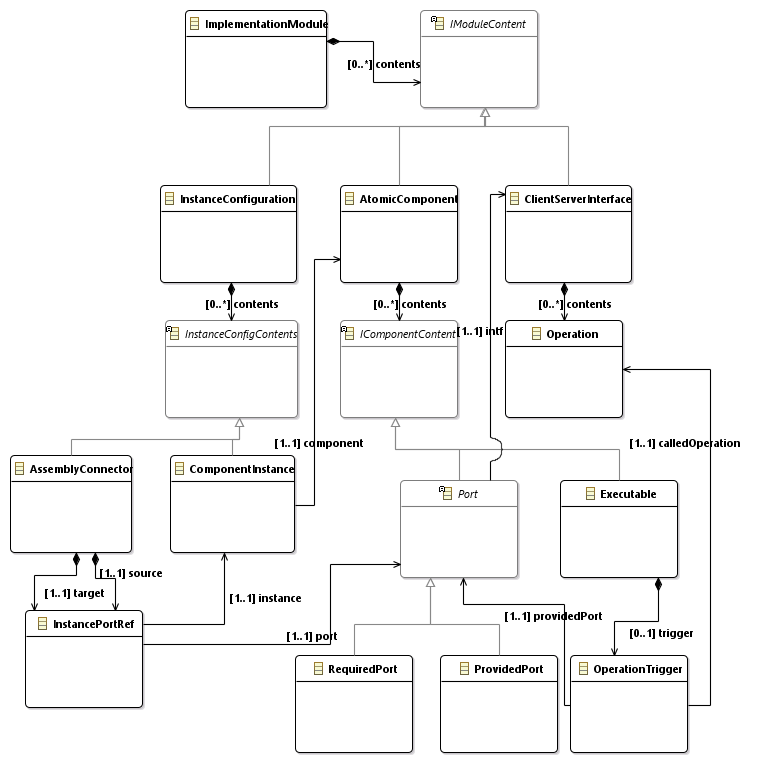
\includegraphics[width=0.48\textwidth]{figures/Moduleclassdiagram}
  \caption{Simplified mbeddr metamodel. \cgg{This picture needs to be compressed.}}
  \label{fig:Moduleclassdiagram}
\end{center}
\end{figure}

The simplified version of the C metamodel is shown in Figure~\ref{fig:CModelclassdiagram}. 
We have included only the concepts that are relevant for the contract we prove in this case study.
A C model has multiple compilation units, which we call ImplementationModules. An ImplementationModule has TypeDefs, StructDeclarations, FunctionPrototypes, Functions and GlobalVariableDeclarations.
In Listing~\ref{code:components_sample_c}, the ImplementationModule has five StructDeclarations, six GlobalVariableDeclarations and seven Functions.
The \verb=Client_i_t= structure has a CFunctionPointerStructMember named \verb=client_process=. The remaining concepts should be familiar to the reader\cgg{Should I give more details about the C or can I assume that they know C?}.

\begin{figure}
\begin{center}
  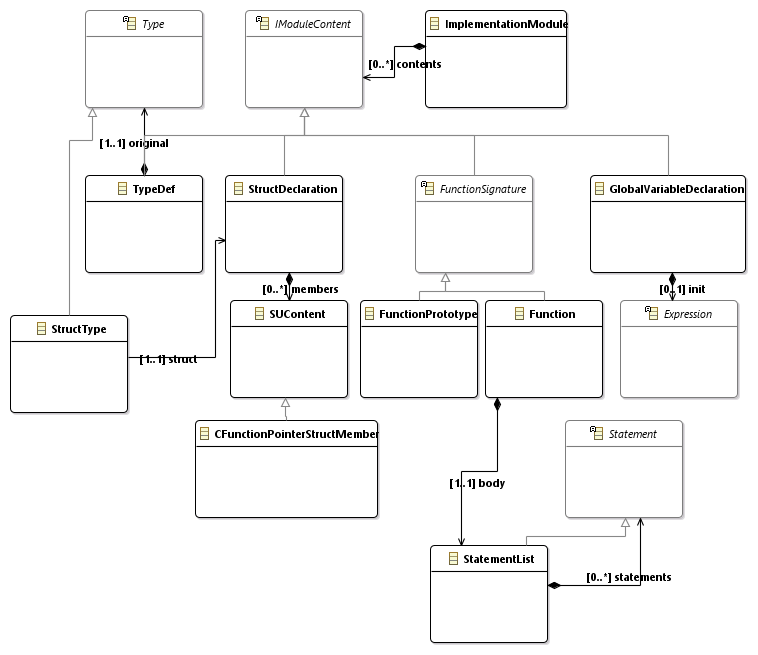
\includegraphics[width=0.48\textwidth]{figures/CModelclassdiagram}
  \caption{Simplified C metamodel. \cgg{This picture needs to be compressed.}}
  \label{fig:CModelclassdiagram}
\end{center}
\end{figure}


\subsubsection{Code Generation}

% Why did we not use the default C code generator and disclaimer
Mbeddr comes with a default C code generator specified in a template language. Unfortunately, we are not able to apply our proof technique to that template language because of its expressivity. Instead, we created an DSLTrans transformation that performs the same task as the generator and in this case study we demonstrate that that transformation is correct with respect to the contract presented before about the correct wiring of the component instances.
We reinforce that the way the C code is generated is exactly the way the default C code generator outputs. We did not decide on how the C code is generated.

% Why did we not use ATL instead of DSLTrans.
We could have specified the generator in declarative ATL~\cite{Jouault2006a}, since it is now supported by SyVolt \cite{Oakes}, but at the time we developed this case study, only DSLTrans was supported.

% Informal description of transformation
By comparing the mbeddr model example in Listing~\ref{code:components_sample_c} with the corresponding generated C code in Listing~\ref{code:simple_example_mbeddr}, we can already hint some informal mappings:
\begin{compactitem}
\item A struct declaration, ending in \verb=_i_t= is created for each ClientServerInterface. This structure holds a pointer for each operation declared in the interface.
\item A struct, ending in \verb=_c_t= is created for each AtomicComponent. This structure has two members for each required port in the component: one to keep the instance of the components that provides that port and the other to hold the reference to the operations that are provided in that port.
\item For each ProvidedPort of each ComponentInstance, there is a global variable ending in \verb=_ops= that will hold references to the implementations of the operations provided in that port.
\item For each operation implemented by a component through a provided port, there is a global function with the code that corresponds to that implementation.
\item There is an \verb=init= operation that call all the wiring functions.
\item And there is a \verb=_wire= function for each component instance. The wiring functions are responsible for two things: initialize the \verb=_ops= global variable with the pointers for the provided operations' implementations; and, in the case of an instance that has a required port that is connected to another instance's provided port, assign the addresses of the target instance's instance and operations to the source instance data.
\end{compactitem}

% Formal description of first layer and justify the trimming of the transformation
The DSLTrans transformation that generates the C model from any mbeddr model has  7 layers and 49 rules. Due to its size, we will focus our discussion in a trimmed version of it, relevant to the contract we are going to prove.
Figure~\ref{fig:mb2c_layer_0} shows the first layer (Layer 0) of the transformation. Rule 1 is creating a StructDeclaration for each ClientServerInterface it finds in the mbeddr model. 
The name of this newly created StructDeclaration is the name of the ClientServerInterface followed by \verb=_i_t=.
Furthermore, the newly create StructDeclaration is traced back to the ClientServerInterface that generated it by a trace named ClientServerStructIData. 
Rule 11 is creating a FunctionPrototype for each Operation declared by the Interface of each ProvidedPort. The name of this Function, although omitted to save space, is a concatenation of the name of the AtomicComponent, name of the ProvidedPort and the name of the Operation. because this FunctionPrototype is associated with the ImplementationModule in later layers (hence, it is in the global scope), this naming ensures no collisions occur.
The other rules in this layer are very similar so we refrain ourselves from explaining them.

\begin{figure}
\begin{center}
  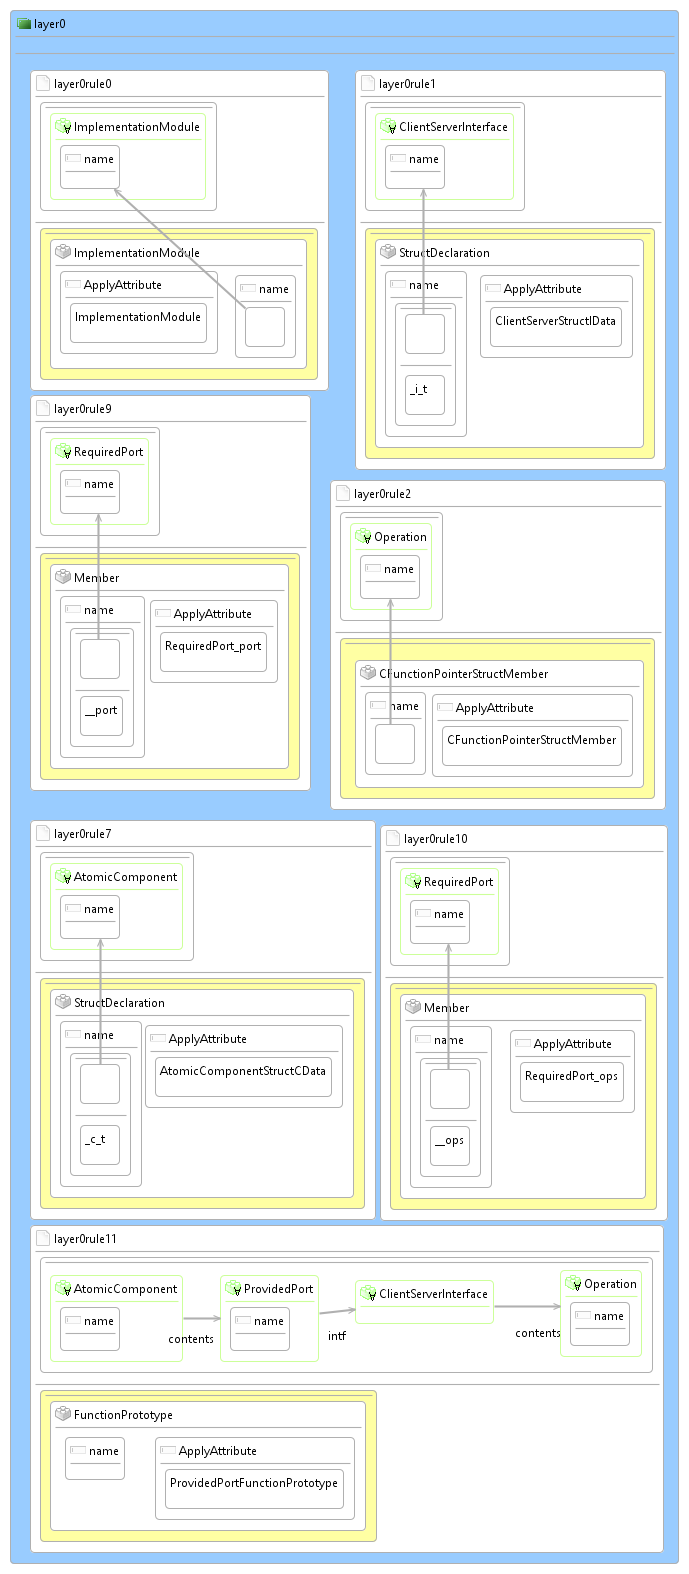
\includegraphics[width=0.48\textwidth]{figures/mbeddr2C_optimized_layer_0}
  \caption{Mbeddr-to-C transformation: layer 0.}
  \label{fig:mb2c_layer_0}
\end{center}
\end{figure}

% layer 1
In the second layer (Layer 1) of the transformation, shown in Figure~\ref{fig:mb2c_layer_1}, the previously created StructDeclaration elements are associated with the ImplementationModule that was created in Layer 0 (Rule 0).
Also, in Rule 12 of this layer, the FunctionPrototype created in the Rule 11 of the previous layer is associated with the ImplementationModule.
The other rules are similar.

\begin{figure}
\begin{center}
  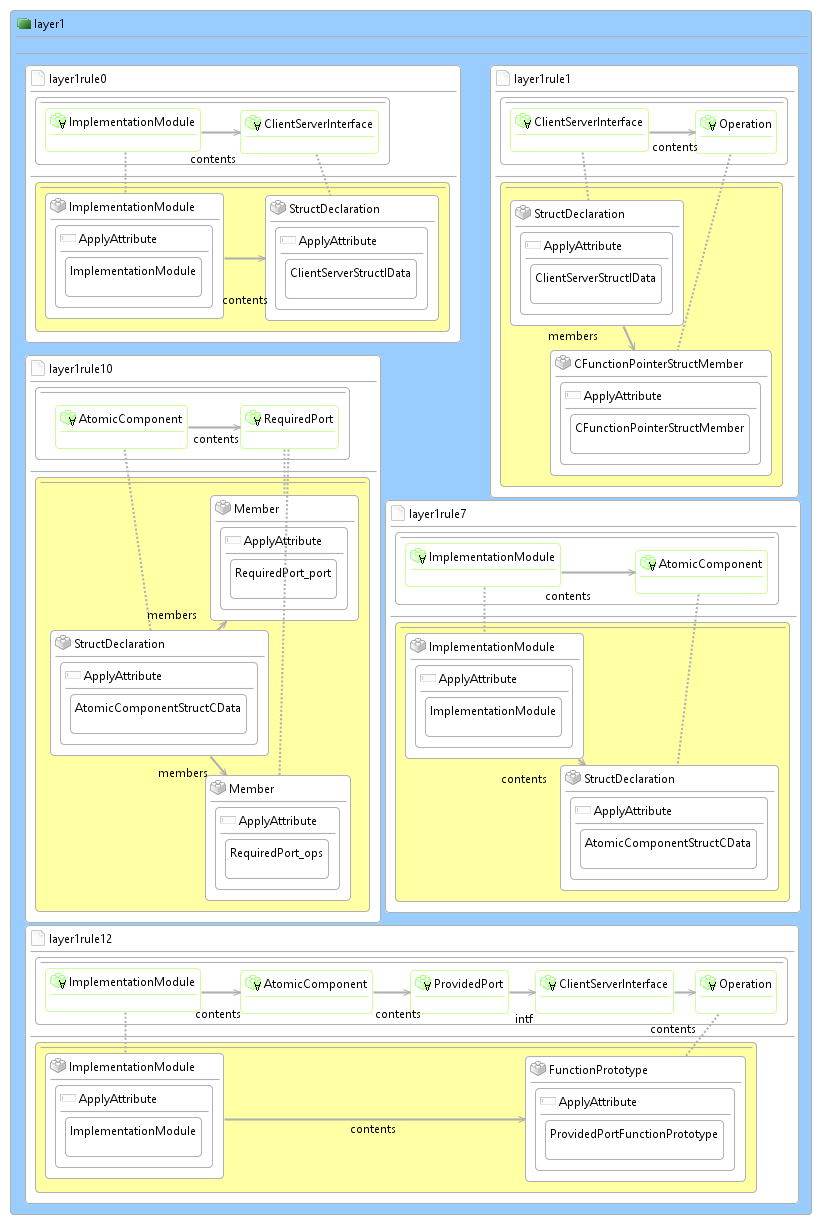
\includegraphics[width=0.48\textwidth]{figures/mbeddr2C_optimized_layer_1}
  \caption{Mbeddr-to-C transformation: layer 1.}
  \label{fig:mb2c_layer_1}
\end{center}
\end{figure}

% layer 3
In Layer 3, Figure~\ref{fig:mb2c_layer_3}, Rule 4 creates a GlobalVariableDeclaration (ended in \verb=_inst=) for each ComponentInstance.
Rule 3 creates a GlobalVariableDeclaration for each ProvidedPort of each ComponentInstance, ended in \verb=_ops=.
These variables will hold the the instance data of the component instance and the address of the provided ports' operations of the component instance.

\begin{figure}
\begin{center}
  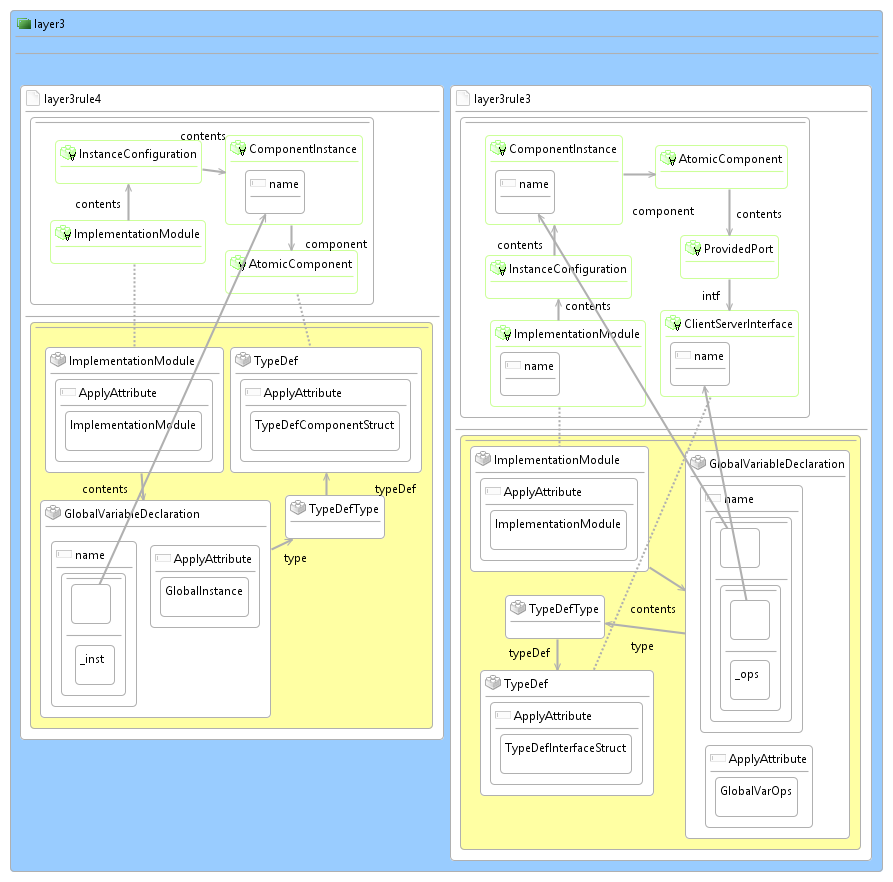
\includegraphics[width=0.48\textwidth]{figures/mbeddr2C_optimized_layer_3}
  \caption{Mbeddr-to-C transformation: layer 3.}
  \label{fig:mb2c_layer_3}
\end{center}
\end{figure}

% Layer 4
The next layer, Layer 4, Figure~\ref{fig:mb2c_layer_4}, creates the \verb=_wire= (Rule 0)
and \verb=init= (Rule 1) Functions from the ComponentInstances and the InstanceConfiguration, respectively. These functions are created with an empty body but they will later implement the wiring of their corresponding component instances. The \verb=init= function will just call all the \verb=_wire= functions.

\begin{figure}
\begin{center}
  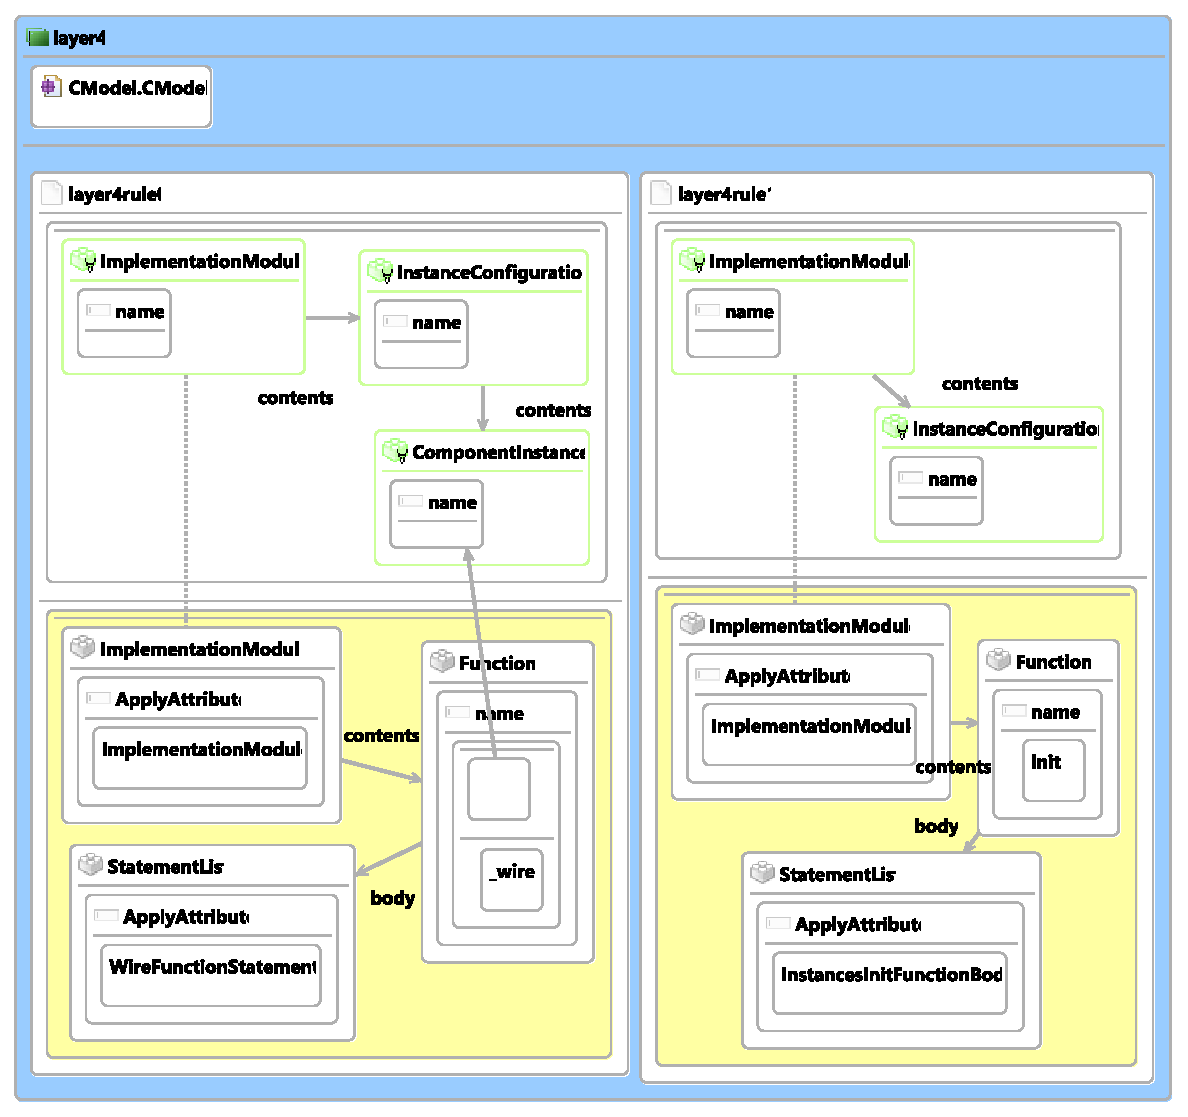
\includegraphics[width=0.48\textwidth]{figures/mbeddr2C_optimized_layer_4}
  \caption{Mbeddr-to-C transformation: layer 4.}
  \label{fig:mb2c_layer_4}
\end{center}
\end{figure}

% Layer 5
Finally, in the last layer, Layer 5, Figure~\ref{fig:mb2c_layer_5},
the bodies of the \verb=init= and \verb=_wire= Functions are filled in.
Rule 0 adds an assignment to the \verb=_wire= Function body that assigns the address of the function prototype created in Rule 11 of Layer 0, to the global variable ended in \verb=_ops=, created in Layer 3, Rule 3.
This assignment is not connecting a provided port with a required port: it is just saving the concrete function implementation in the \verb=_ops= variable.
The connection is made in Rule 1 of this layer. The match pattern is complex but it is essentially capturing all the relevant entities that surround an AssemblyConnector: the source and target component instances and their provided/required ports. When a match for this rule is found, two assignments are added to the \verb=_wire= function of the source component instance:
one to assign the address of the global variable that holds the instance data of the target component instance; and one to assign the address of the variable that holds the operations of the provided port to a member of the structure that folds the required port operations of the source component instance.
Rule 2 is just adding to the body of the \verb=init=, a function call to each of the \verb=_wire= functions.

\begin{figure}
\begin{center}
  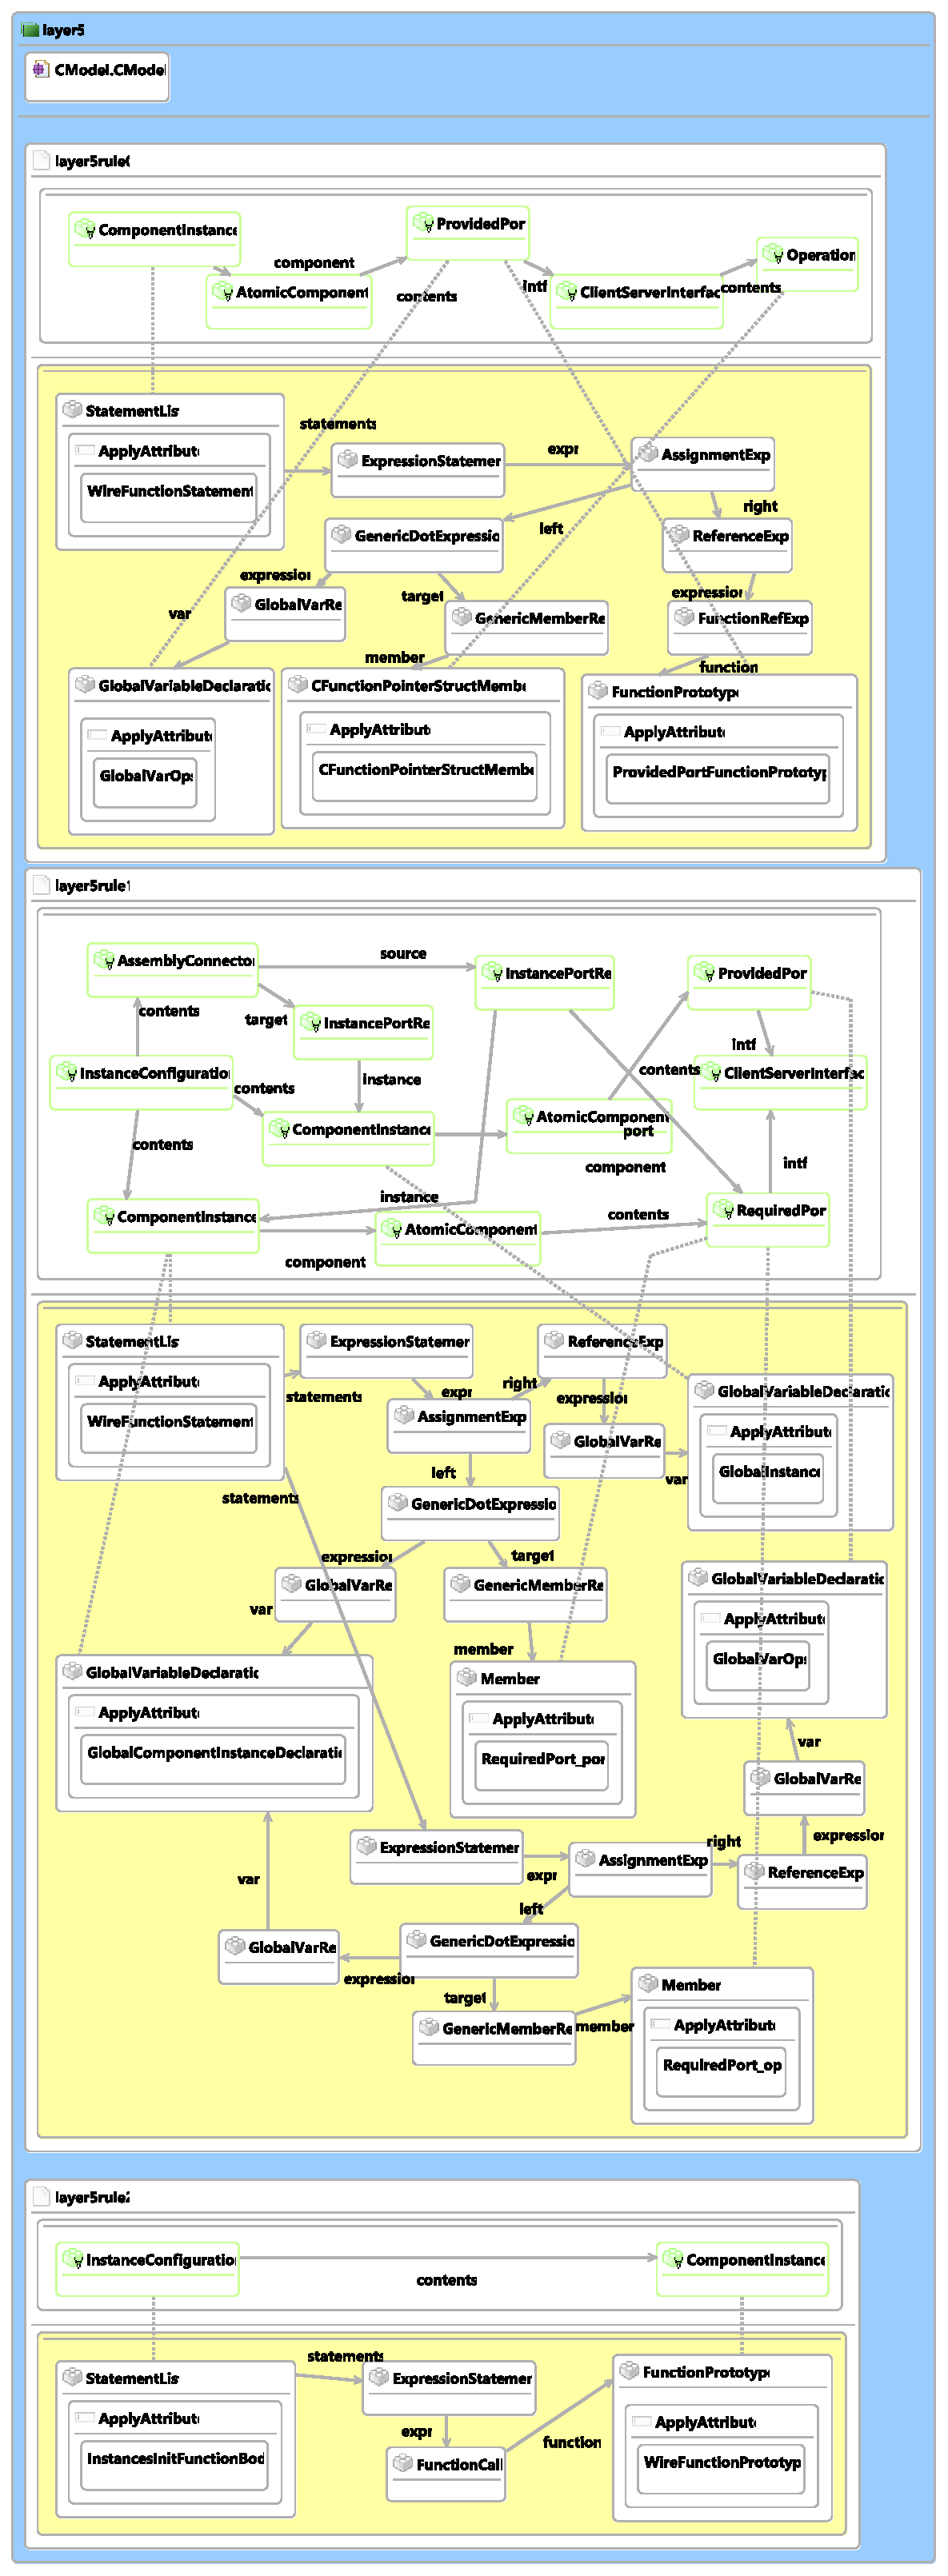
\includegraphics[width=0.48\textwidth]{figures/mbeddr2C_optimized_layer_5}
  \caption{Mbeddr-to-C transformation: layer 5.}
  \label{fig:mb2c_layer_5}
\end{center}
\end{figure}


\subsection{Correct Code Generation}

% pre-requisites for correctness.

In order for the transformation we just described to be correct, the wiring of instances must be correct. The pre-requisites for this are:
\begin{compactenum}
\item The pointers to the provided port operations, assigned to the instance variable that requires those operations do really point to the corresponding operations.
\item The correct pointers are assigned to the correct instance variable.
\item Besides in the wiring function, that is called by the initialization function, the instance variables' member that contains the provided port operation reference is not assigned anywhere else.
\item The same thing as the previous for the pointers.
\end{compactenum}
\cgg{The above discussion is incomplete. I need to discuss this with Levi and Bentley and I need the SyVolt property.}























